\documentclass{article}
\usepackage{indentfirst}
\setlength{\parindent}{2em}
\usepackage{graphicx}

\title{SYSC 5001W: Project deliverable 3} % Title of the assignment

\author{Qiguang Chu\\ \texttt{300042722}} % Author name and email address

\date{University of Ottawa --- \today} % University, school and/or department name(s) and a date

%----------------------------------------------------------------------------------------

\begin{document}

\maketitle

\section{Data Collection}

The first thing we need to consider after model translation is data collection. For the supply of components are infinite,  the input I formulate here is \textbf{the output of two inspectors}. There are five channels output of two inspectors and three kinds of components totally. So I extract data from Inspector's inspection time for components. Each data point represents the time of a specific component processed. I identify the distributions of each set of data using histograms. Below is what I draw by using python matplotlib library. Obviously, the distributions fit the exponential PDF curve well. 
\begin{figure}[htbp]
\begin{center}
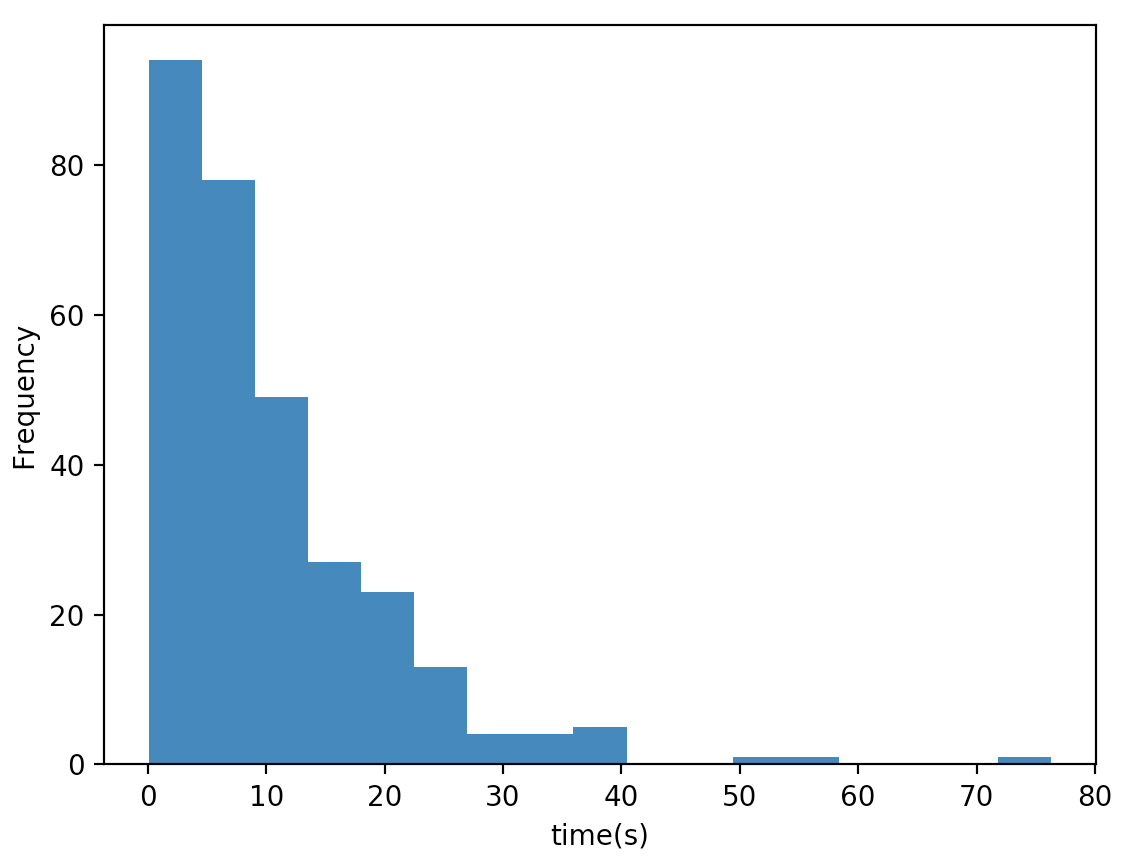
\includegraphics[width=2in]{dataCollection1.png}
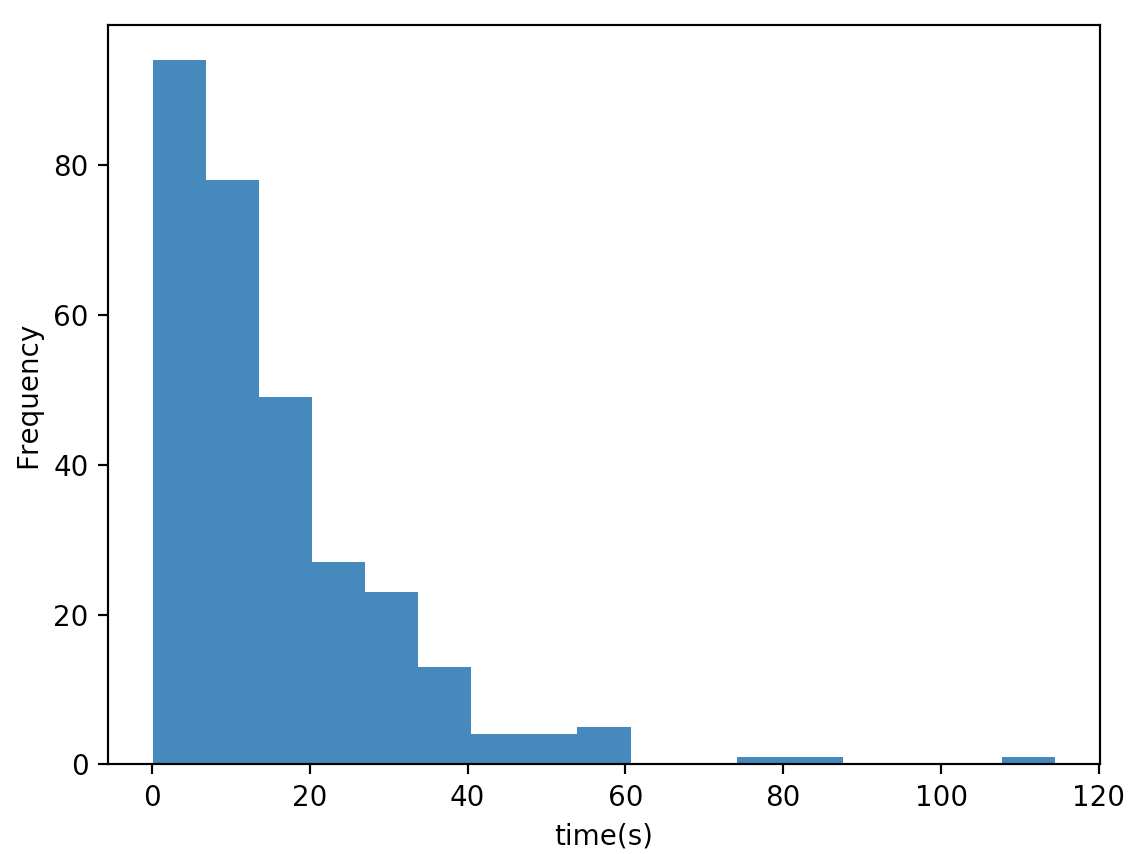
\includegraphics[width=2in]{dataCollection2.png}
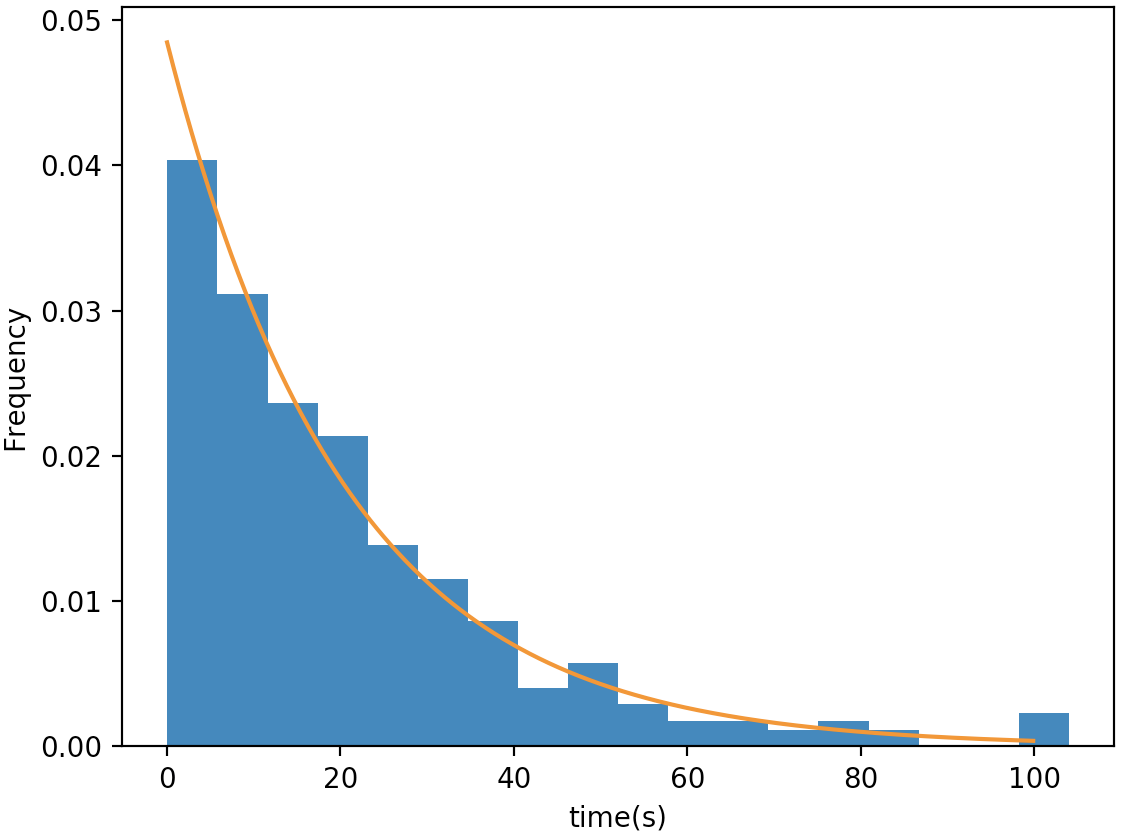
\includegraphics[width=2in]{dataCollection3.png}
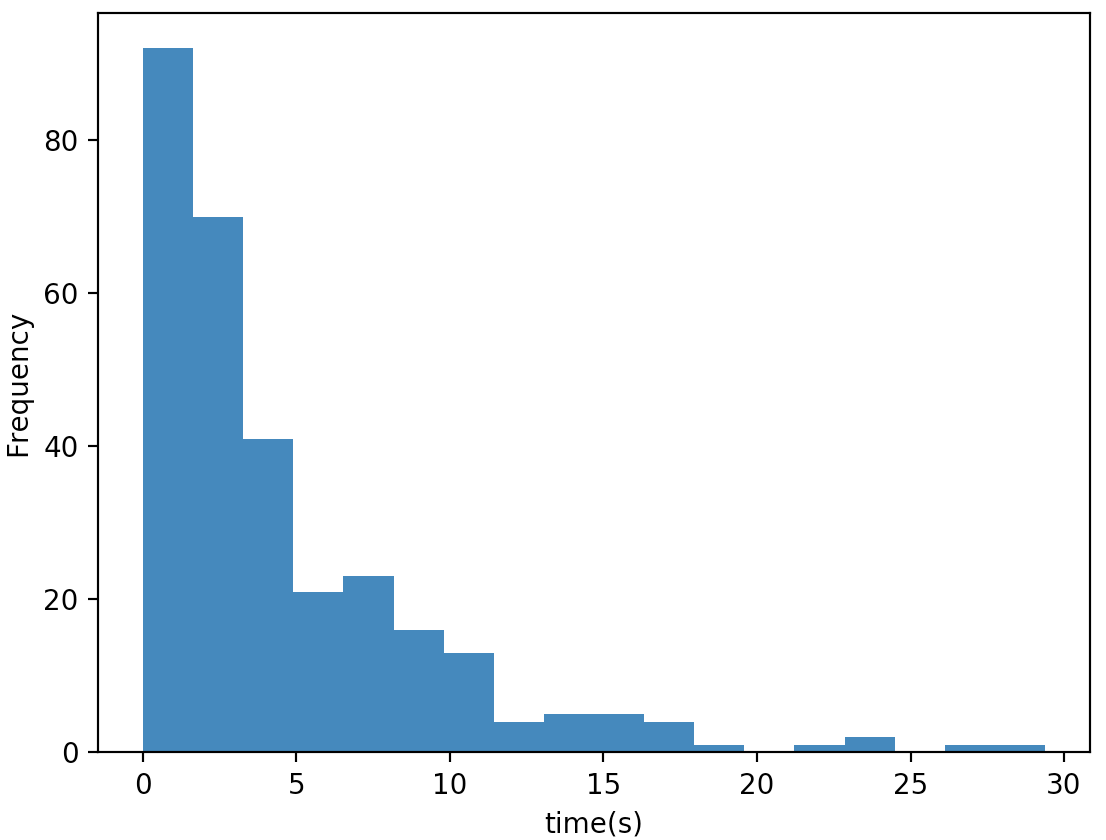
\includegraphics[width=2in]{dataCollection4.png}
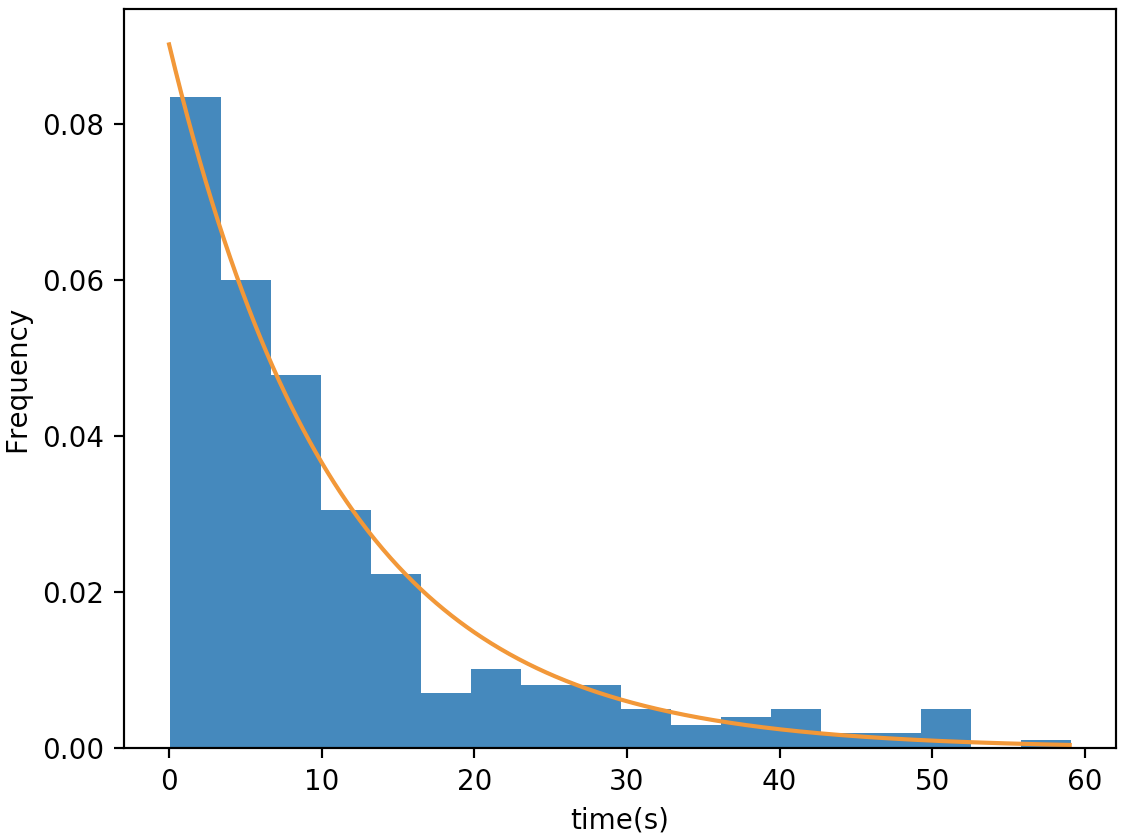
\includegraphics[width=2in]{dataCollection5.png}
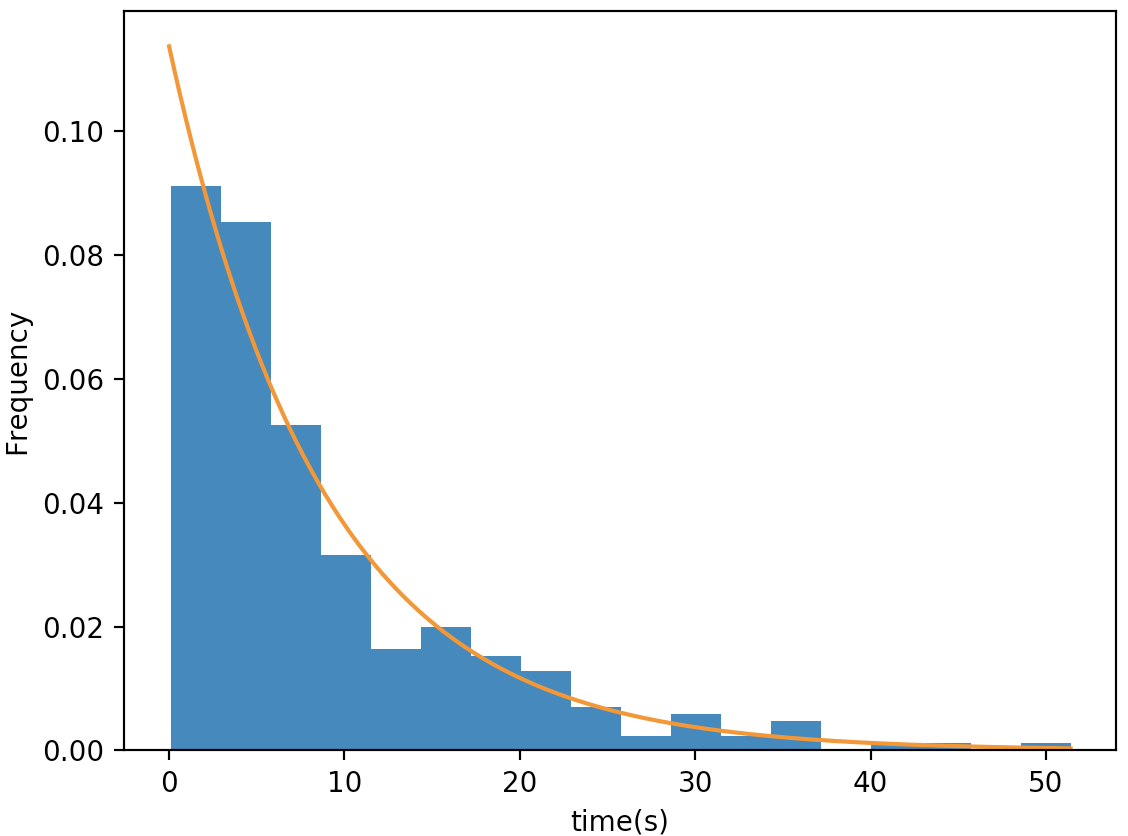
\includegraphics[width=2in]{dataCollection6.png}
\caption{Data collection of 3 Inspectors and 3 Workstations}
\label{data}
\end{center}
\end{figure}

I choose exponential distribution to do a fitting and it seems good.

\begin{figure}[htbp]
\begin{center}
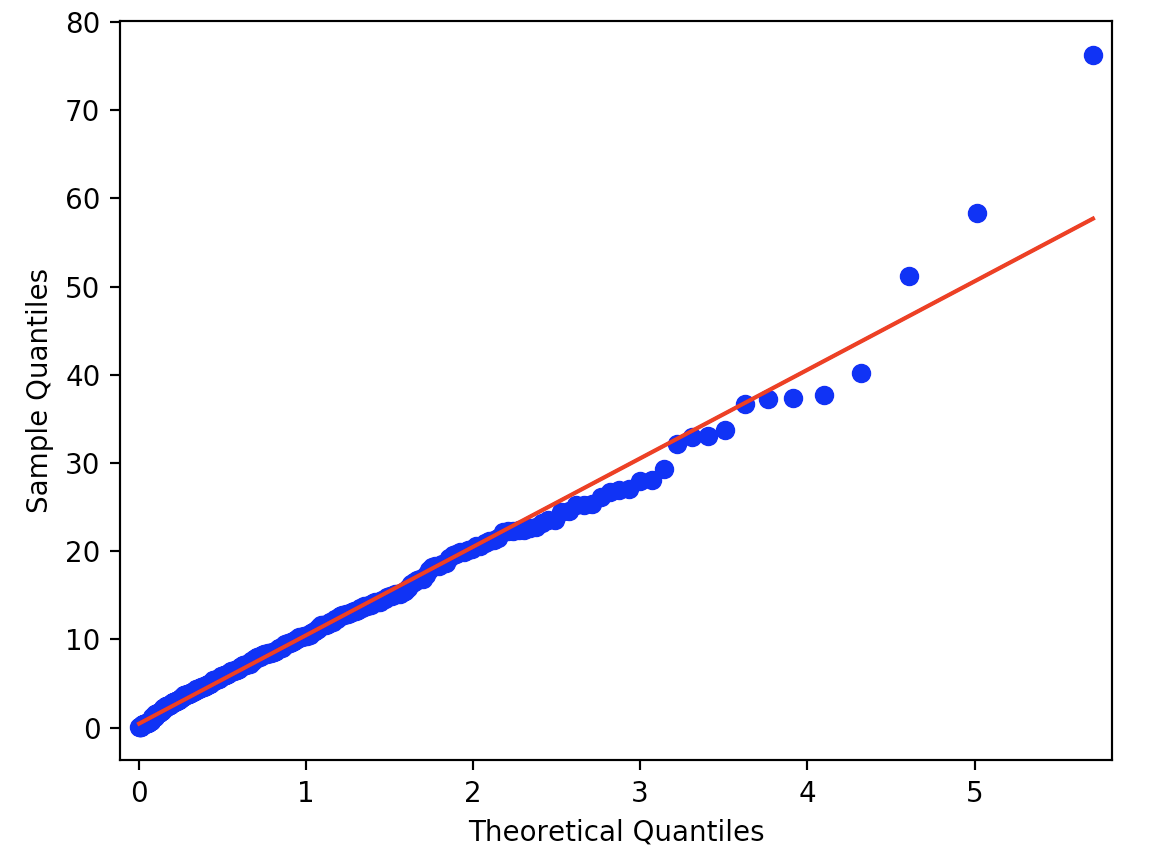
\includegraphics[width=2in]{hist1.png}
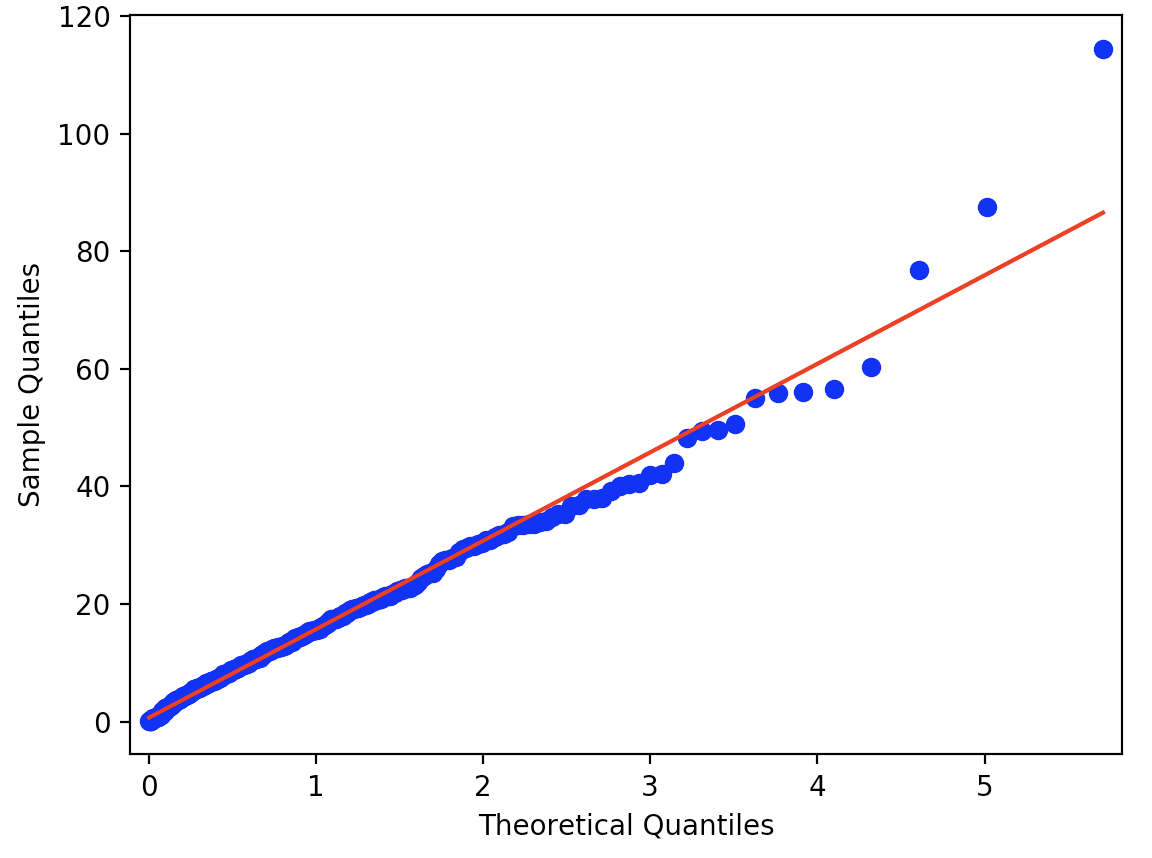
\includegraphics[width=2in]{hist2.png}
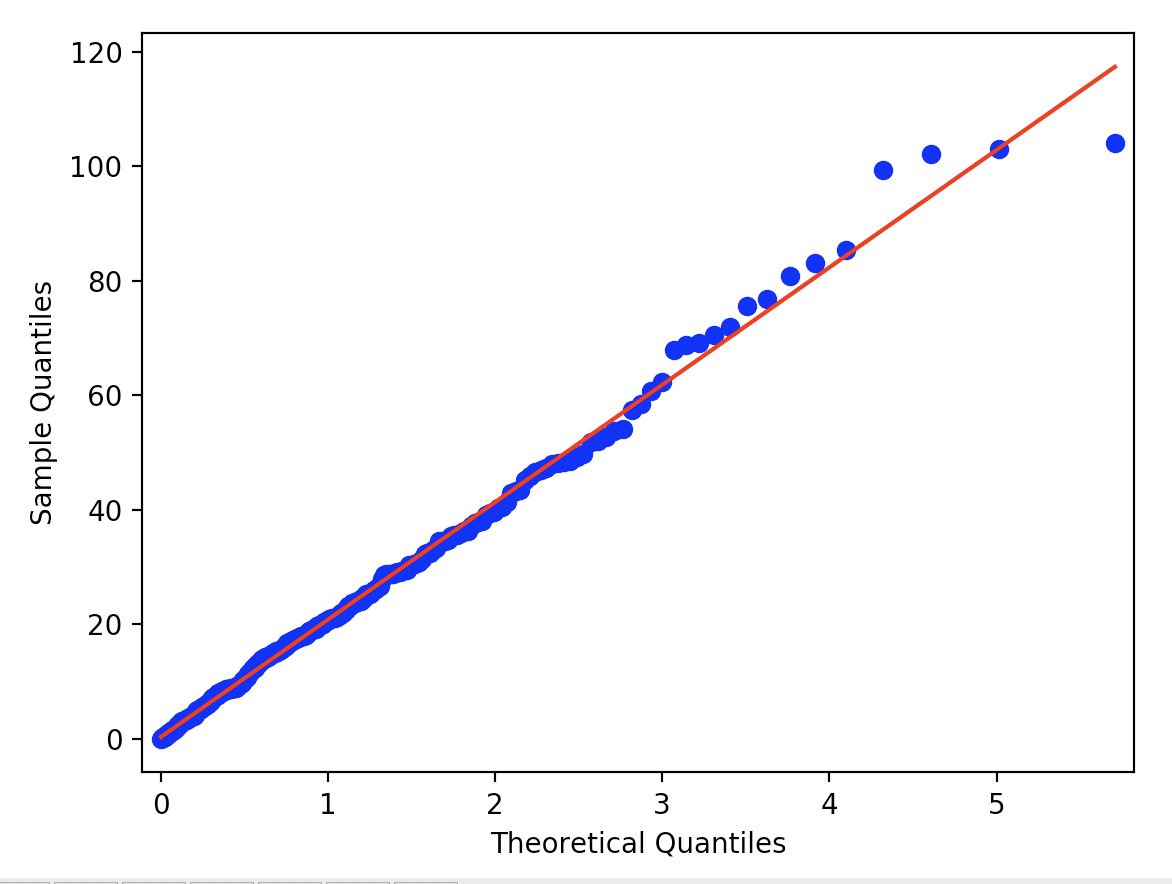
\includegraphics[width=2in]{hist3.png}
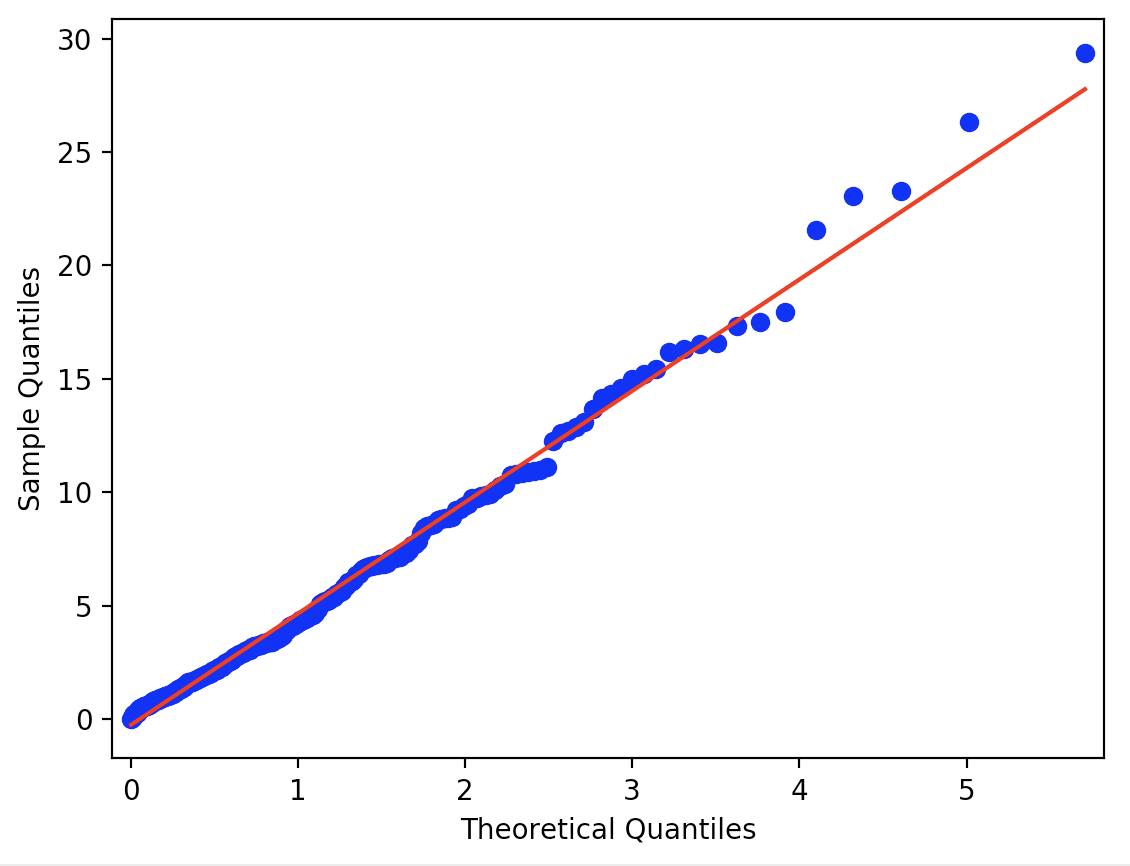
\includegraphics[width=2in]{hist4.png}
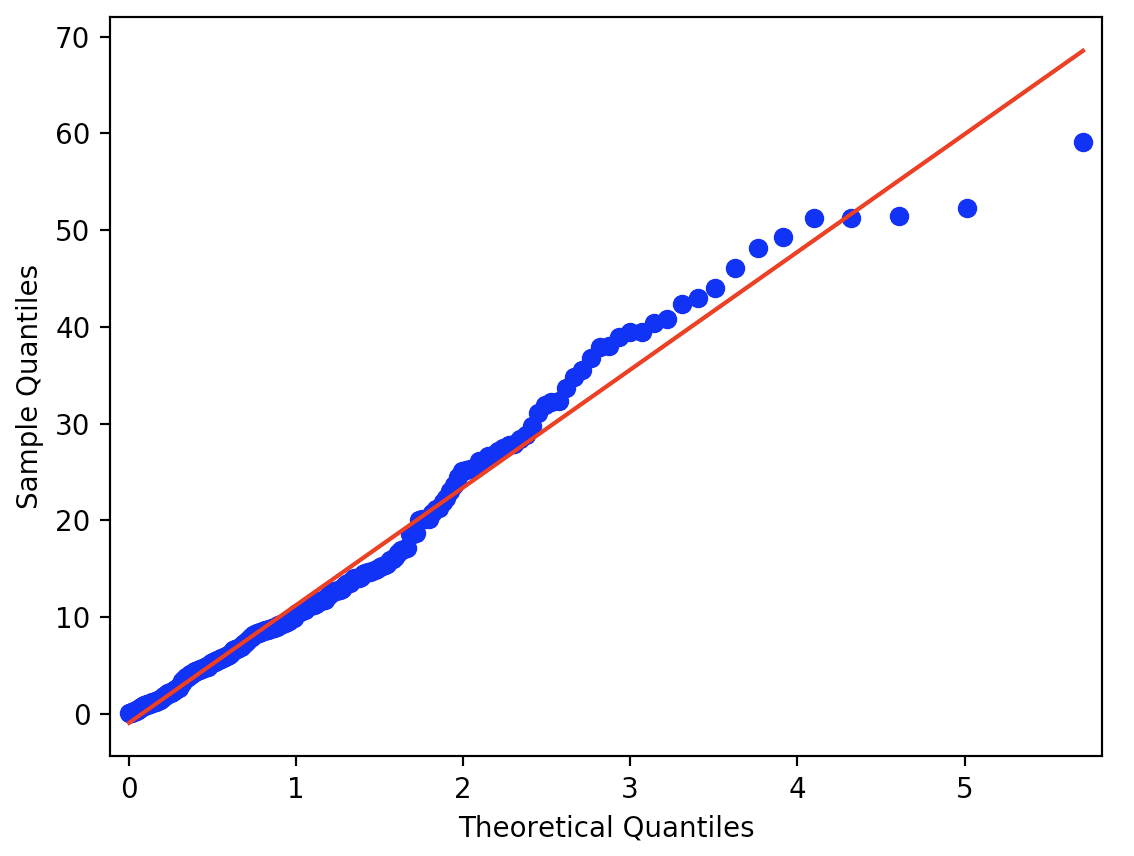
\includegraphics[width=2in]{hist5.png}
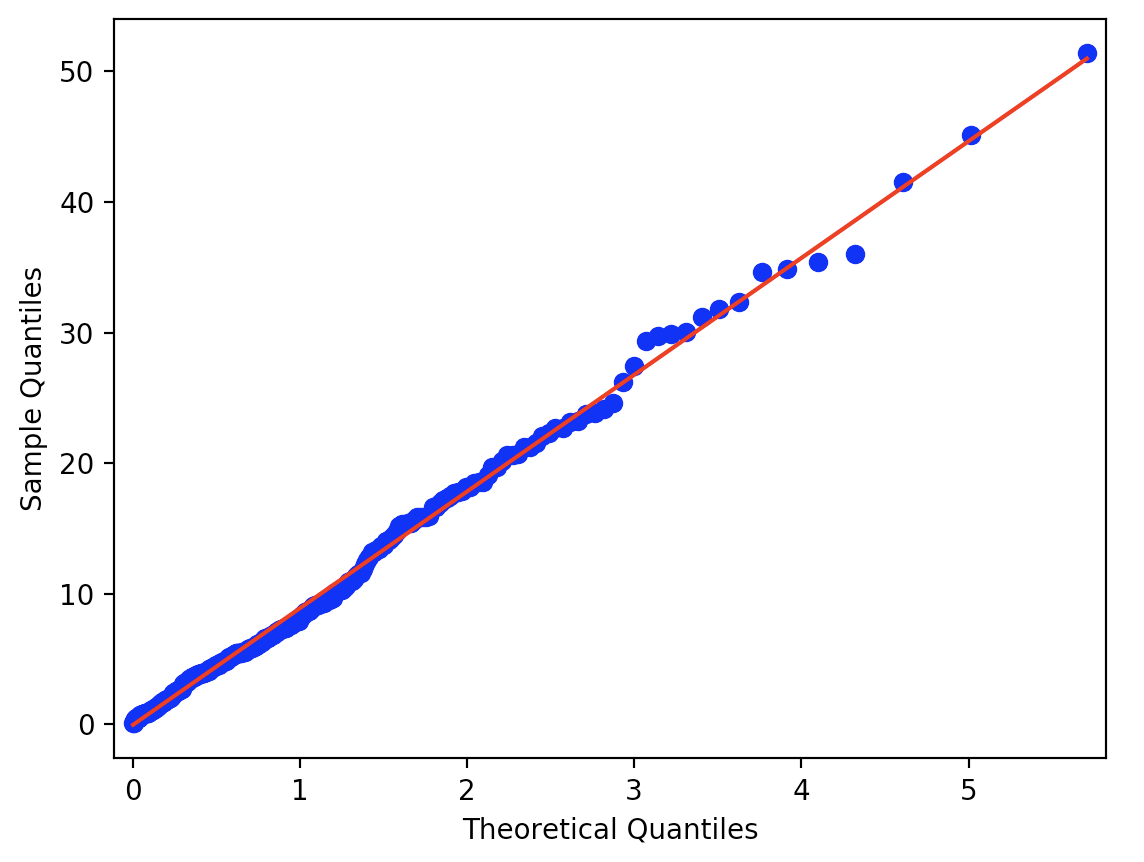
\includegraphics[width=2in]{hist6.png}
\caption{Fitting of normal exponential distribution with distributions of 3 Inspectors and 3 Workstations}
\label{data2}
\end{center}
\end{figure}

\section{Q-Q plots}

The construction of histograms are necessary ingredients for choosing a family of distribution but it's not as useful to evaluate the fit of chosen distribution. Quantile-quantile plot is a useful tool for evaluating distribution fit.

First let ${\{x_i, i=1,2,...,n\}}$ be sampled data and sort the from the smallest to the largest ${\{y_j, j=1,2,...,n\}}$. The $q-q$ plot is based on that $y_i$ is an estimate of the $(j-1/2)/n$ quantile of sampled data. I set $\sqrt{300} = 18$ bins totally.

\begin{figure}[htbp]
\begin{center}
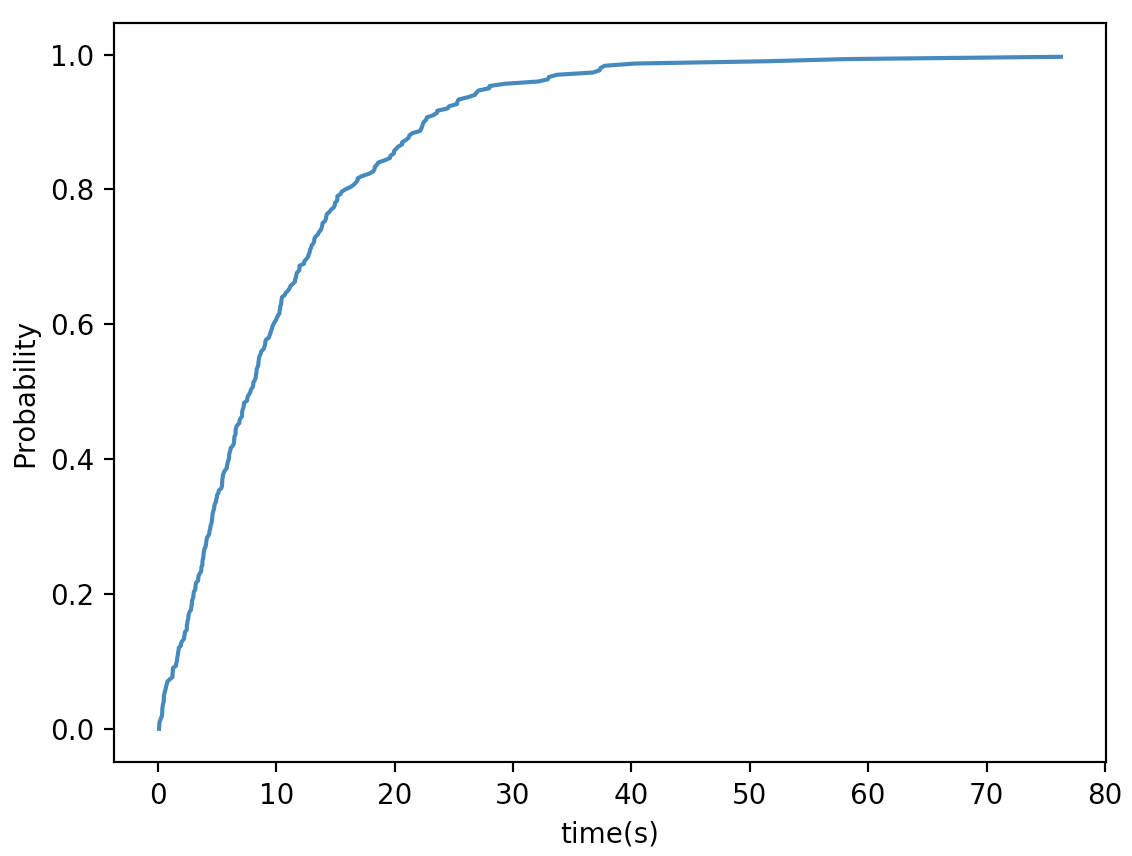
\includegraphics[width=2in]{cdf1.png}
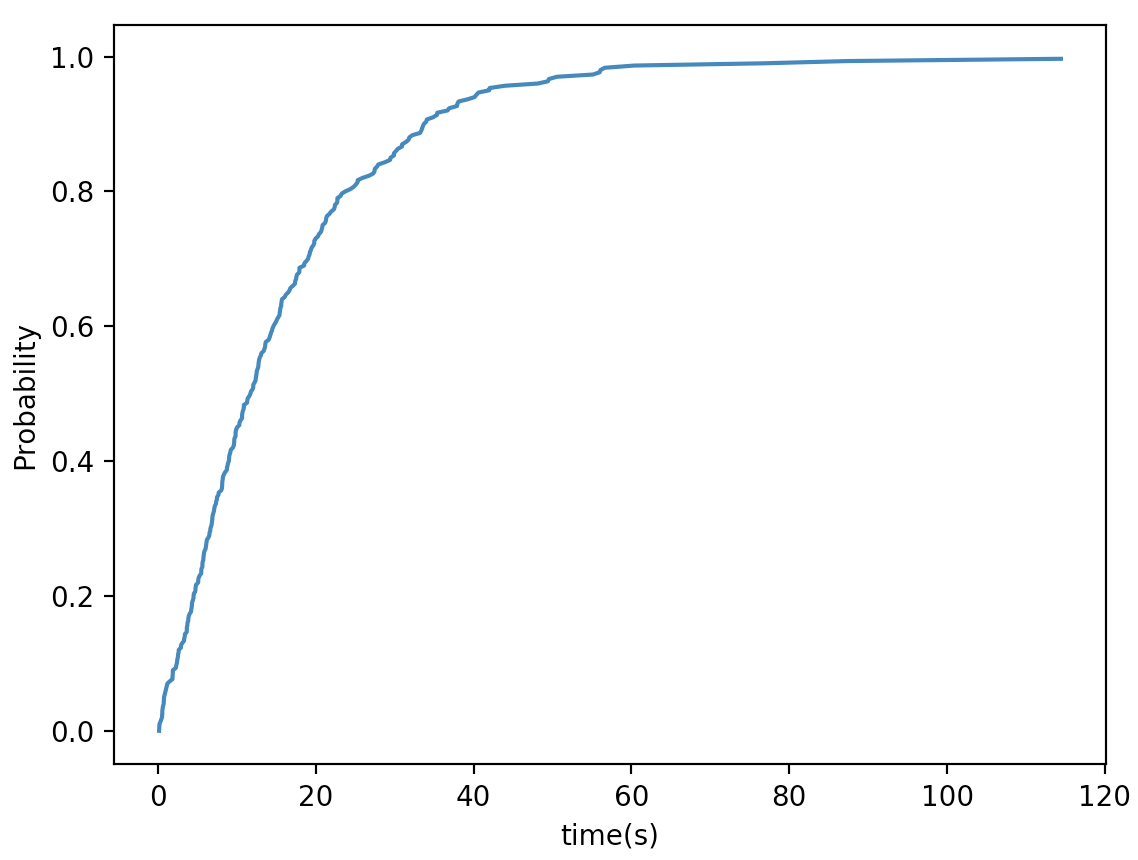
\includegraphics[width=2in]{cdf2.png}
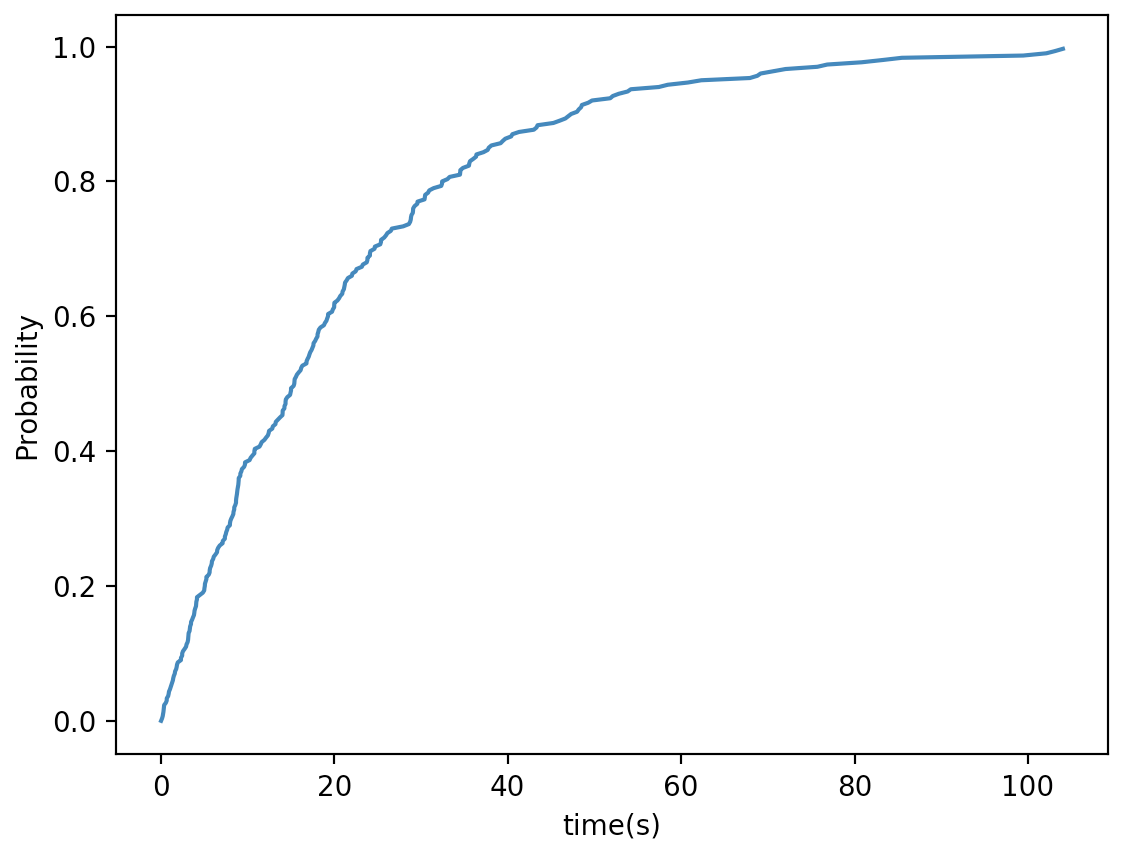
\includegraphics[width=2in]{cdf3.png}
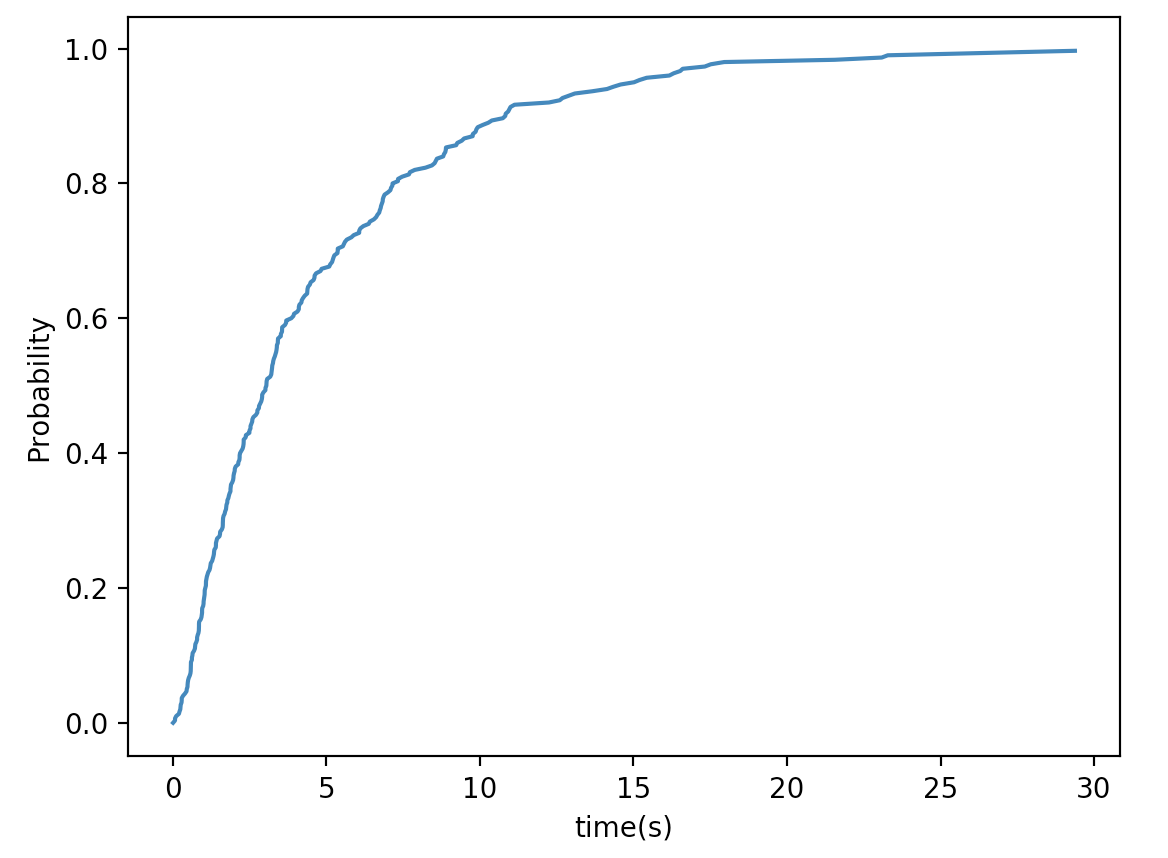
\includegraphics[width=2in]{cdf4.png}
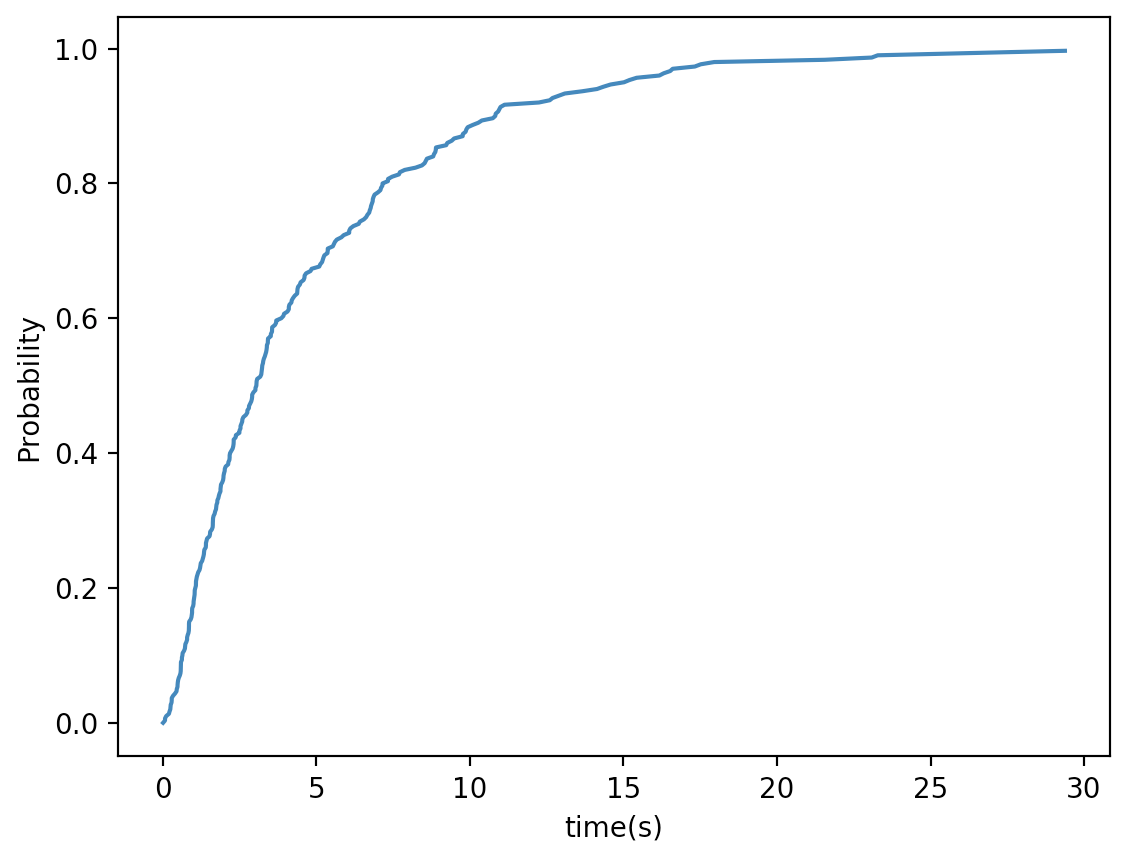
\includegraphics[width=2in]{cdf5.png}
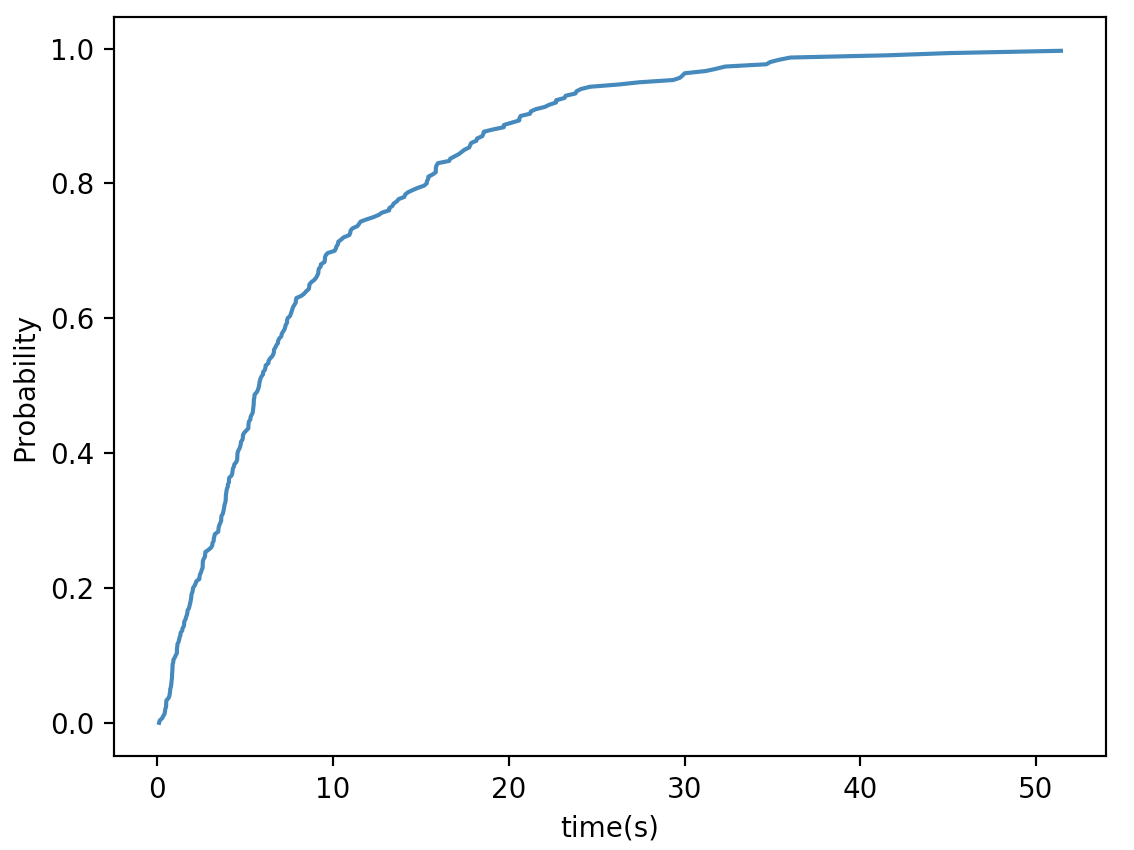
\includegraphics[width=2in]{cdf6.png}
\caption{CDF of 3 Inspectors and 3 Workstations}
\label{cdf}
\end{center}
\end{figure}
Try some different kinds of common distribution and I found exponential distribution fits the most.
Below I choose exponential distribution as the family.


\section{Chi-Square Test}
\subsection{Component1 from Inspector1}
The following hypotheses are formed;

$H_0$: The random variable is exponential distributed.
$H_1$: The random variable is not exponential distributed.

the pmf for exponential distribution is given:

\begin{equation}
p(x) = \left\{
\begin{array}{rl}
\lambda e^{-\lambda e}, x\geq 0\\
0, x<0
\end{array}
\right.
\end{equation}

We assume that $\hat{\lambda}=\frac{1}{\bar{X}}=0.097$
\begin{table}[htp]
\caption{Chi-Square Goodness-of-Fit Test}
\begin{center}
\begin{tabular}{ccccc}
\hline
$x_i$ & Class Interval & $Observed\ Frequency$ & $Expected\ Frequency$ & $\frac{(O_i-E_i)^2}{E_i}$\\
0& [0, 0.4238)&87&100.74&1.87\\
1& [4.238, 8.476)&79&66.91&2.18\\
2&[8.476, 12.714)&46&44.44&0.05\\
3& [12.714, 16.952)&34&29.52&0.68\\
4&[16.952, 21.19)&19&19.61&0.02\\
5& [21.19, 25.428)&16&13.02&0.68\\
6& [25.428, 29.666)&7&8.65&0.31\\
7& [29.666, 33.904)&4&5.75&0.53\\
8& [33.904, 38.142)&4&3.82&0.01\\
9& [38.142, 42.38)&1&2.53&0.93\\
10&[42.38, 46.618)&0&1.68&1.68\\
11&[46.618, 50.856)&0&1.12&1.12\\
12& [50.856, 55.094)&1&0.74&0.09\\
13& [55.094, 59.332)&1&0.49&0.52\\
14& [59.332, 63.57)&0&0.33&0.33\\
15& [63.57, 67.808)&0&0.22&0.22\\
16& [67.808, 72.046)&0&0.14&0.14\\
17& [72.046, 76.284]&1&0.10&8.51\\
18& (76.284, $\infty$)&0&0.19&0.19\\
\hline
Total& &300&300&20.08\\

\hline

\end{tabular}
\end{center}
\label{default}
\end{table}%

We have 18 bins and the freedom degree should be 18-1-1=16. Using a significance level of 0.05 and check the table, we find that $\chi^2_{0.05, 16}=26.3 > 20.09$. So we can't reject that the input follows exponential distribution.

\subsection{Component2 from Inspector2}

We assume that $\hat{\lambda}=\frac{1}{\bar{X}}=0.097$
\begin{table}[htp]
\caption{Chi-Square Goodness-of-Fit Test}
\begin{center}
\begin{tabular}{ccccc}
\hline
$x_i$ & Class Interval & $Observed\ Frequency$ & $Expected\ Frequency$ & $\frac{(O_i-E_i)^2}{E_i}$\\
0& [0, 6.357)&87&100.74&1.87\\
1& [6.357, 12.714)&79&66.91&2.18\\
2&[12.714, 19.071)&46&44.44&0.05\\
3& [19.071, 25.428)&34&29.52&0.68\\
4&[25.428, 31.785)&19&19.61&0.02\\
5&[31.785, 38.142)&16&13.02&0.68\\
6&[38.142, 44.499)&7&8.65&0.31\\
7&[44.499, 50.856)&4&5.75&0.53\\
8&[50.856, 57.213)&4&3.82&0.01\\
9&[57.213, 63.57)&1&2.53&0.93\\
10&[63.57, 69.927)&0&1.68&1.68\\
11&[69.927, 76.284)&0&1.12&1.12\\
12&[76.284, 82.641)&1&0.74&0.09\\
13&[82.641, 88.998)&1&0.49&0.52\\
14&[88.998, 95.355)&0&0.33&0.33\\
15&[95.355, 101.712)&0&0.22&0.22\\
16&[101.712, 108.069)&0&0.14&0.14\\
17&[108.069, 114.426]&1&0.10&8.51\\
18& (114.426, $\infty$)&0&0.19&0.19\\
\hline
Total& &300&300&20.08\\

\hline

\end{tabular}
\end{center}
\label{default}
\end{table}%

We have 18 bins and the freedom degree should be 18-1-1=16. Using a significance level of 0.05 and check the table, we find that $\chi^2_{0.05, 16}=26.3 > 20.06$. So we can't reject that the input follows exponential distribution.

\subsection{Component3 from Inspector2}

We assume that $\hat{\lambda}=\frac{1}{\bar{X}}=0.048$
\begin{table}[htp]
\caption{Chi-Square Goodness-of-Fit Test}
\begin{center}
\begin{tabular}{ccccc}
\hline
$x_i$ & Class Interval & $Observed\ Frequency$ & $Expected\ Frequency$ & $\frac{(O_i-E_i)^2}{E_i}$\\
0&[0, 5.7788)&70&73.28&0.15\\
1&[5.7788, 11.5576)&54&55.38&0.03\\
2&[11.5576, 17.3364)&41&41.85&0.02\\
3&[17.3364, 23.1152)&37&31.63&0.91\\
4&[23.1152, 28.894)&24&23.90&0\\
5&[28.894, 34.6728)&20&18.06&0.21\\
6&[34.6728, 40.4516)&15&13.65&0.13\\
7&[40.4516, 46.2304)&7&10.32&1.07\\
8&[46.2304, 52.0092)&10&7.80&0.62\\
9&[52.0092, 57.788)&5&5.89&0.14\\
10&[57.788, 63.5668)&3&4.45&0.47\\
11&[63.5668, 69.3456)&3&3.37&0.04\\
12&[69.3456, 75.1244)&2&2.54&0.12\\
13&[75.1244, 80.9032)&3&1.92&0.60\\
14&[80.9032, 86.682)&2&1.45&0.21\\
15&[86.682, 92.4608)&0&1.10&1.10\\
16&[92.4608, 98.2396)&0&0.83&0.83\\
17&[98.2396, 104.0184]&4&0.63&18.15\\
18&(104.0184, $\infty$)&0&0.01&0.01\\
\hline
Total& &300&300&24.80\\

\hline

\end{tabular}
\end{center}
\label{default}
\end{table}%

We have 18 bins and the freedom degree should be 18-1-1=16. Using a significance level of 0.05 and check the table, we find that $\chi^2_{0.05, 16}=26.3 > 24.8$. So we can't reject that the input follows exponential distribution.



\subsection{Workstation1}

We assume that $\hat{\lambda}=\frac{1}{\bar{X}}=0.217$
\begin{table}[htp]
\caption{Chi-Square Goodness-of-Fit Test}
\begin{center}
\begin{tabular}{ccccc}
\hline
$x_i$ & Class Interval & $Observed\ Frequency$ & $Expected\ Frequency$ & $\frac{(O_i-E_i)^2}{E_i}$\\
0&[0, 1.6319)&92&89.53&0.07\\
1&[1.6319, 3.2638)&70&62.81&0.82\\
2&[3.2638, 4.8957)&41&44.07&0.21\\
3&[4.8957, 6.5276)&21&30.92&3.18\\
4&[6.5276, 8.1595)&23&21.69&0.08\\
5&[8.1595, 9.7914)&16&15.22&0.04\\
6&[9.7914, 11.4233)&13&10.67&0.51\\
7&[11.4233, 13.0552)&4&7.49&1.63\\
8&[13.0552, 14.6871)&5&5.25&0.01\\
9&[14.6871, 16.319)&5&3.69&0.47\\
10&[16.319, 17.9509)&4&2.59&0.77\\
11&[17.9509, 19.5828)&1&1.81&0.37\\
12&[19.5828, 21.2147)&0&1.27&1.27\\
13&[21.2147, 22.8466)&1&0.89&0.01\\
14&[22.8466, 24.4785)&2&0.63&3.01\\
15&[24.4785, 26.1104)&0&0.44&0.44\\
16&[26.1104, 27.7423)&1&0.31&1.55\\
17&[27.7423, 29.3742]&1&0.22&2.84\\
18&(29.3742, $\infty$)&0&0.51&0.51\\
\hline
Total& &300&300&17.79\\

\hline

\end{tabular}
\end{center}
\label{default}
\end{table}%

We have 18 bins and the freedom degree should be 18-1-1=16. Using a significance level of 0.05 and check the table, we find that $\chi^2_{0.05, 16}=26.3 > 17.79$. So we can't reject that the input follows exponential distribution.


\subsection{Workstation2}
We assume that $\hat{\lambda}=\frac{1}{\bar{X}}=0.217$
\begin{table}[htp]
\caption{Chi-Square Goodness-of-Fit Test}
\begin{center}
\begin{tabular}{ccccc}
\hline
$x_i$ & Class Interval & $Observed\ Frequency$ & $Expecte\ Frequency$ & $\frac{(O_i-E_i)^2}{E_i}$\\
0&[0, 3.2821)&82&76.85&0.34\\
1&[3.2821, 6.5642)&59&57.17&0.06\\
2&[6.5642, 9.8463)&47&42.52&0.47\\
3&[9.8463, 13.1284)&30&31.63&0.08\\
4&[13.1284, 16.4105)&22&23.53&0.10\\
5&[16.4105, 19.6926)&7&17.50&6.30\\
6&[19.6926, 22.9747)&10&13.02&0.70\\
7&[22.9747, 26.2568)&8&9.68&0.30\\
8&[26.2568, 29.5389)&8&7.20&0.09\\
9&[29.5389, 32.821)&5&5.36&0.02\\
10&[32.821, 36.1031)&3&3.98&0.24\\
11&[36.1031, 39.3852)&4&2.96&0.36\\
12&[39.3852, 42.6673)&5&2.20&3.55\\
13&[42.6673, 45.9494)&2&1.64&0.08\\
14&[45.9494, 49.2315)&2&1.22&0.50\\
15&[49.2315, 52.5136)&5&0.91&18.46\\
16&[52.5136, 55.7957)&0&0.67&0.67\\
17&[55.7957, 59.0778]&1&0.50&0.49\\
18&(59.0778, $\infty$)&0&1.46&1.46\\
\hline
Total& &300&300&24.28\\

\hline

\end{tabular}
\end{center}
\label{default}
\end{table}%

We have 18 bins and the freedom degree should be 18-1-1=16. Using a significance level of 0.01 and check the table, we find that $\chi^2_{0.01, 16}=26.3 > 24.28$. So we don't reject that the input follows exponential distribution.

\subsection{Workstation3}

We assume that $\hat{\lambda}=\frac{1}{\bar{X}}=0.217$
\begin{table}[htp]
\caption{Chi-Square Goodness-of-Fit Test}
\begin{center}
\begin{tabular}{ccccc}
\hline
$x_i$ & Class Interval & $Observed\ Frequency$ & $Expected\ Frequency$ & $\frac{(O_i-E_i)^2}{E_i}$\\
0&[0, 3.2821)&78&76.84&0.02\\
1&[3.2821, 6.5642)&73&57.16&4.39\\
2&[6.5642, 9.8463)&45&42.52&0.14\\
3&[9.8463, 13.1284)&27&31.63&0.68\\
4&[13.1284, 16.4105)&14&23.53&3.86\\
5&[16.4105, 19.6926)&17&17.50&0.01\\
6&[19.6926, 22.9747)&13&13.02&0\\
7&[22.9747, 26.2568)&11&9.68&0.18\\
8&[26.2568, 29.5389)&6&7.20&0.20\\
9&[29.5389, 32.821)&2&5.36&2.11\\
10&[32.821, 36.1031)&5&3.98&0.26\\
11&[36.1031, 39.3852)&2&2.96&0.31\\
12&[39.3852, 42.6673)&4&2.20&1.46\\
13&[42.6673, 45.9494)&0&1.64&1.64\\
14&[45.9494, 49.2315)&1&1.22&0.04\\
15&[49.2315, 52.5136)&1&0.91&0.01\\
16&[52.5136, 55.7957)&0&0.67&0.67\\
17&[55.7957, 59.0778]&1&0.50&0.49\\
18&(59.0778, $\infty$)&0&1.46&0.09\\
\hline
Total& &300&300&17.57\\

\hline

\end{tabular}
\end{center}
\label{default}
\end{table}%

We have 18 bins and the freedom degree should be 18-1-1=16. Using a significance level of 0.05 and check the table, we find that $\chi^2_{0.05, 16}=26.3 > 17.57$. So we don't reject that the input follows exponential distribution.

\section{Generate the input}

For each inspector and workstation, we choose a model based on that the sampled input. We choose 0.95 significance level for each and make sure they can all be presented as the distribution. What I do is generating random numbers first in uniform distribution. Then, I put these random numbers into exponential distribution that they are transferred random variables of time.

\begin{itemize}
\item Inspection time for C1:
\begin{equation}
f(x) = \left\{
\begin{array}{rl}
0.0965 e^{-0.0965 e}, x\geq 0\\
0, x<0
\end{array}
\right.
\end{equation}
\item Inspection time for C2:
\begin{equation}
f(x) = \left\{
\begin{array}{rl}
0.0644 e^{-0.0644 e}, x\geq 0\\
0, x<0
\end{array}
\right.
\end{equation}
\item Inspection time for C3:
\begin{equation}
f(x) = \left\{
\begin{array}{rl}
0.0485 e^{-0.0485 e}, x\geq 0\\
0, x<0
\end{array}
\right.
\end{equation}
\item Inspection time for W1:
\begin{equation}
f(x) = \left\{
\begin{array}{rl}
0.217 e^{-0.217 e}, x\geq 0\\
0, x<0
\end{array}
\right.
\end{equation}
\item Inspection time for W2:
\begin{equation}
f(x) = \left\{
\begin{array}{rl}
0.0901 e^{-0.0901 e}, x\geq 0\\
0, x<0
\end{array}
\right.
\end{equation}
\item Inspection time for W3:
\begin{equation}
f(x) = \left\{
\begin{array}{rl}
0.1137 e^{-0.1137 e}, x\geq 0\\
0, x<0
\end{array}
\right.
\end{equation}
\end{itemize}

Here we have generated random numbers data.

\begin{figure}[htbp]
\begin{center}
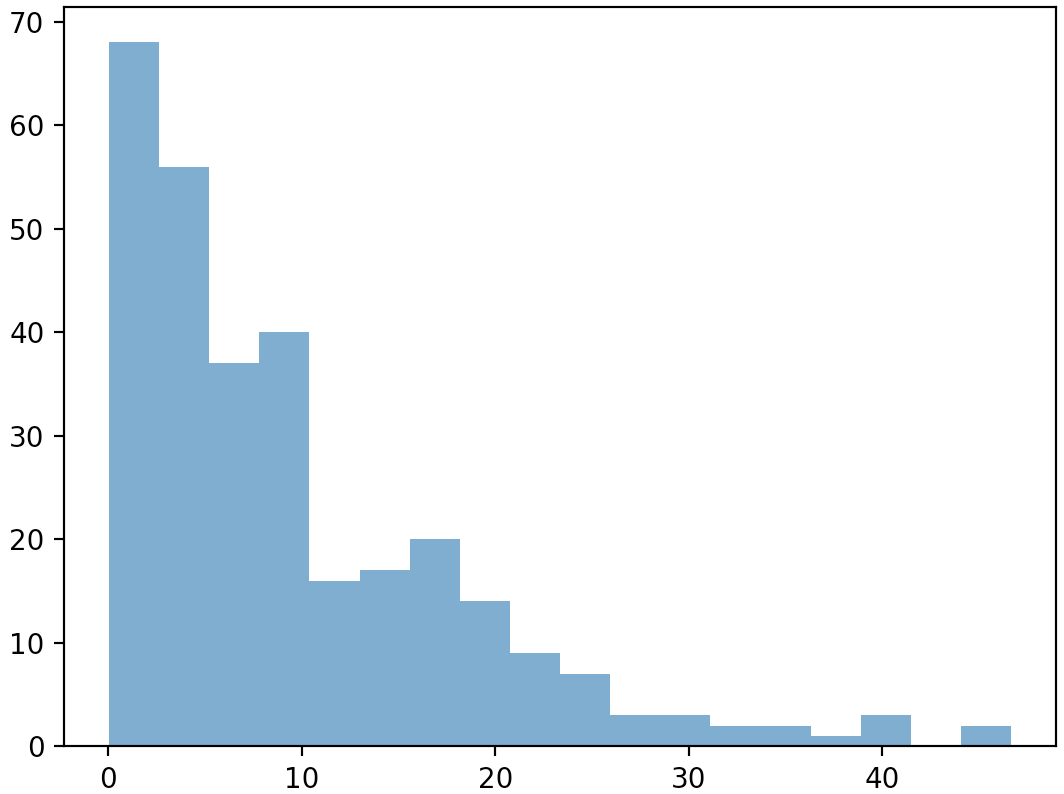
\includegraphics[width=2in]{generate1.png}
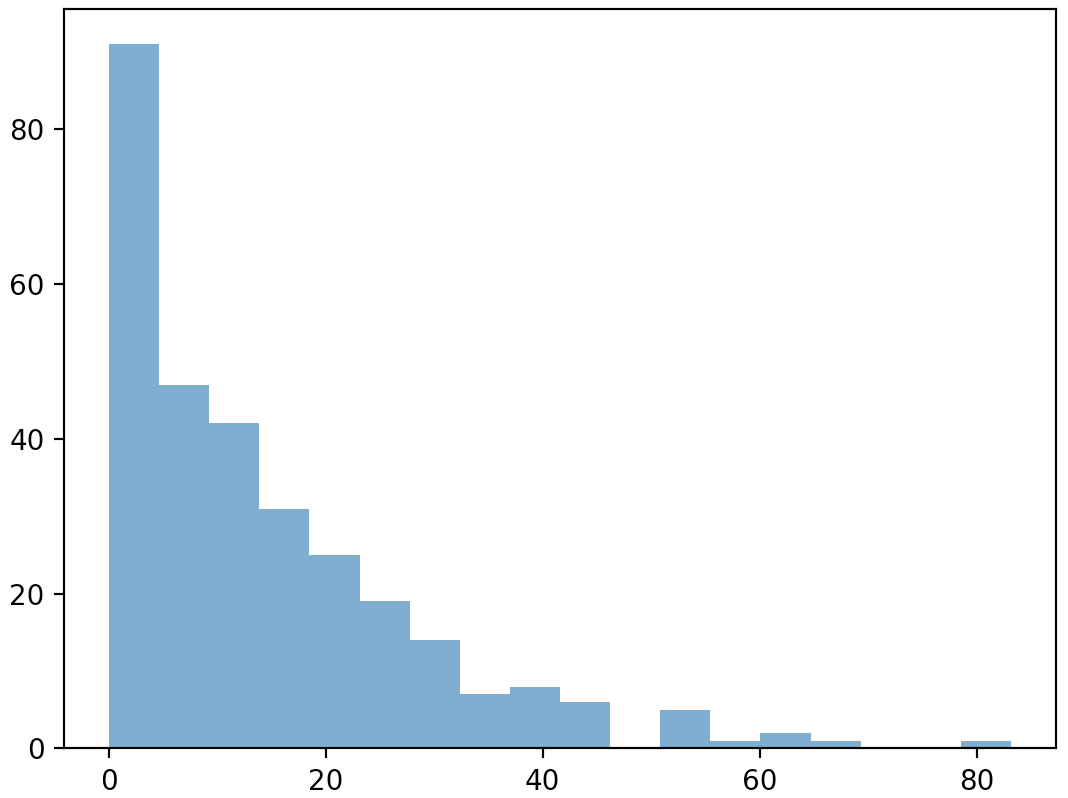
\includegraphics[width=2in]{generate2.png}
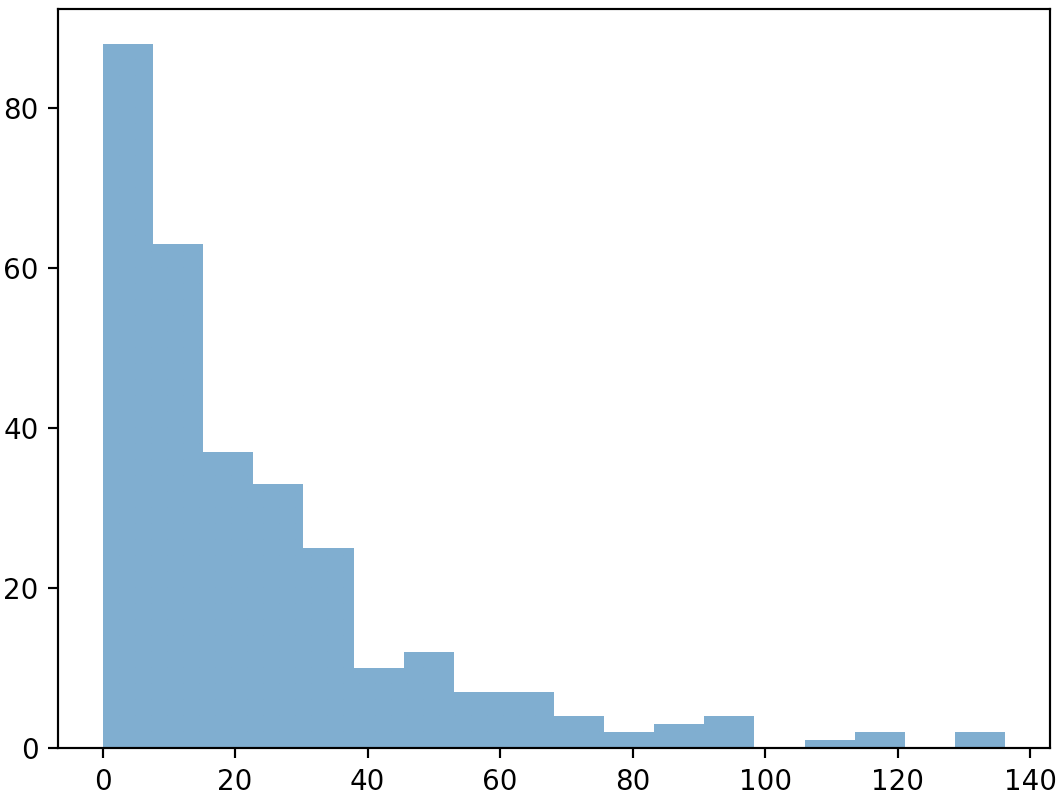
\includegraphics[width=2in]{generate3.png}
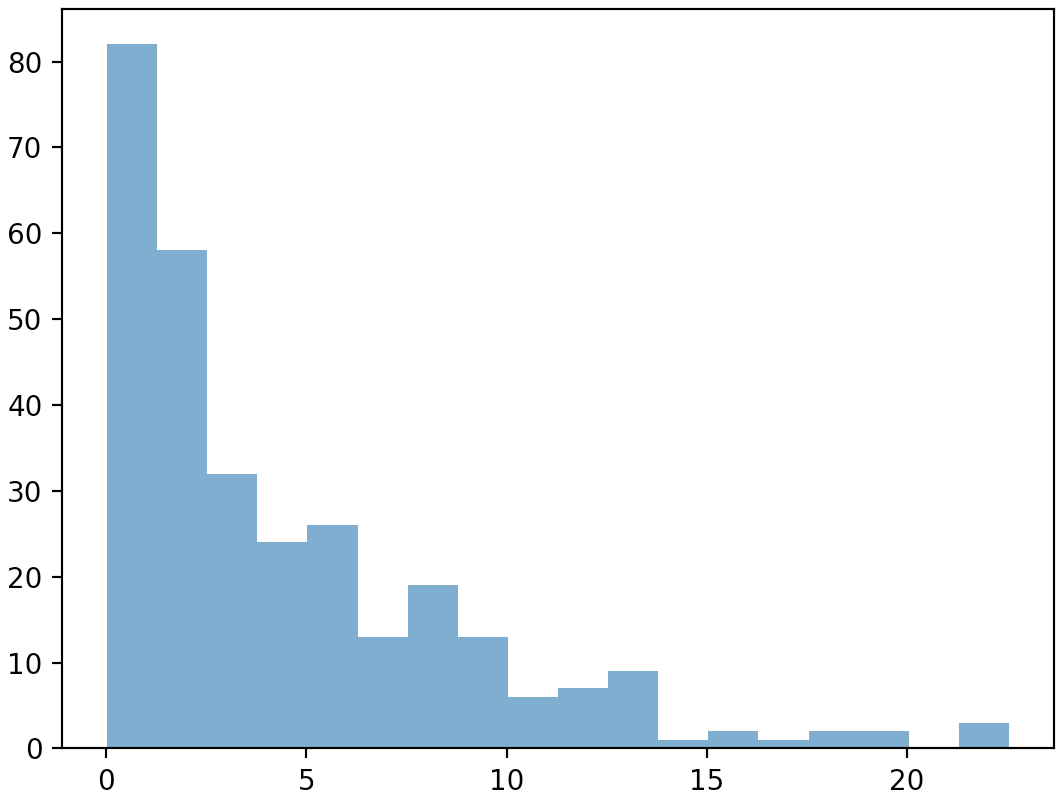
\includegraphics[width=2in]{generate4.png}
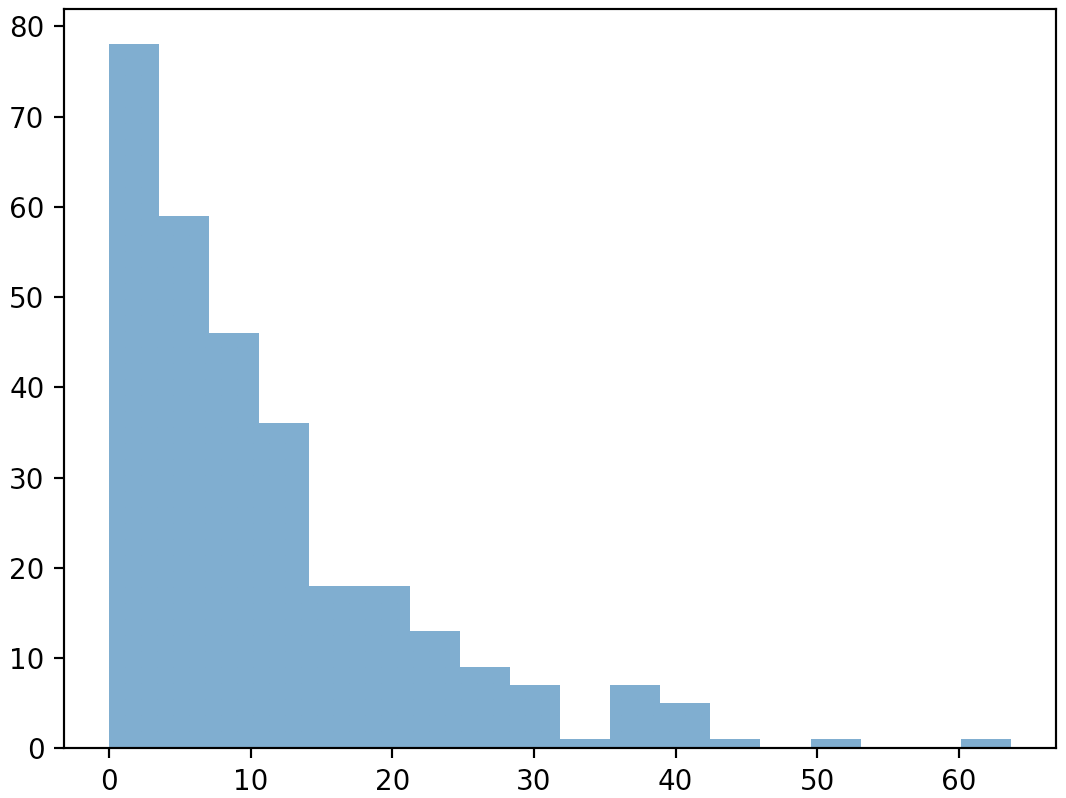
\includegraphics[width=2in]{generate5.png}
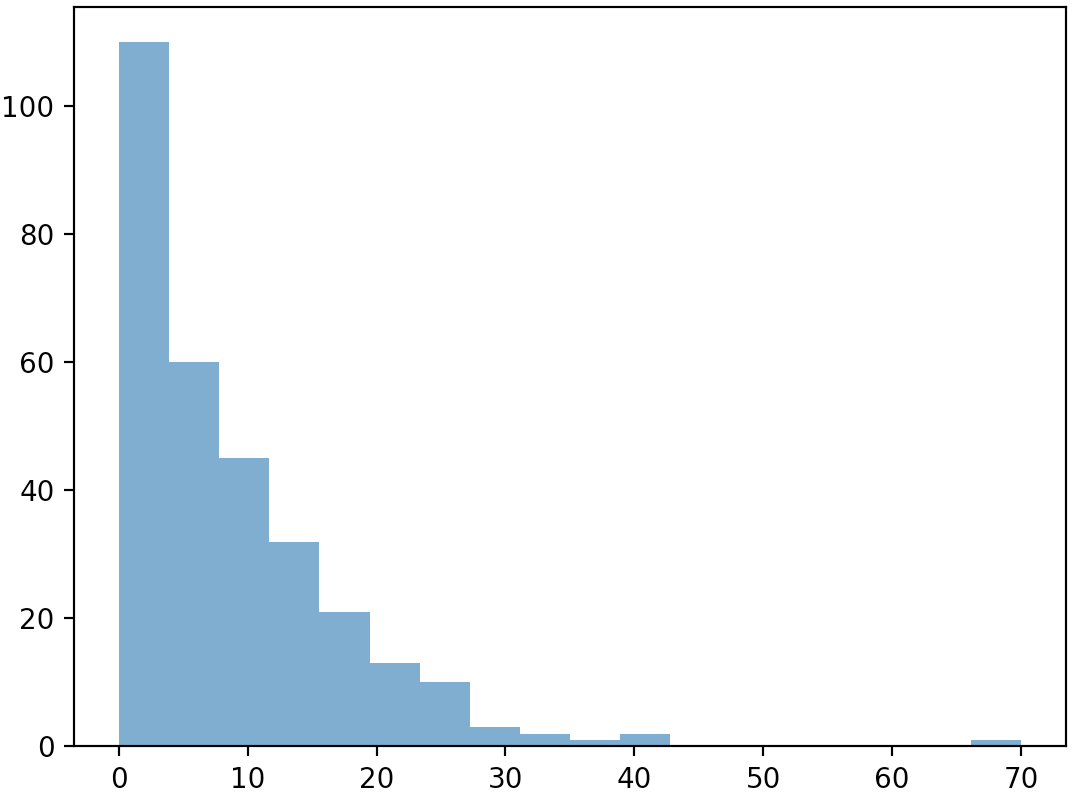
\includegraphics[width=2in]{generate6.png}
\caption{Generated data of 3 Inspectors and 3 Workstations}
\label{data}
\end{center}
\end{figure}




\end{document}